\chapter{検証・評価}
本章では提案したDNA配列アラインメントスコア計算用の光Race Logic回路について機能検証と評価を行う.
\section{検証}
検証に用いたのはOptiwave社が提供するOptisystemというシミュレータである.
OptiSystemは光ネットワークのあらゆるタイプの広範囲のシステムの設計,評価,シミュレーションを行なうソフトウェアである.
素子レベルからシステムレベルまでの物理レイヤー上の光通信システムの設計と解析を行うことができる.

配列長N=2のアラインメントスコアを求める提案回路について,光Race Logic arrayの動作を確認した.
今回のシミュレーションにおいて,各素子において光伝搬信号に影響を与える雑音や損失は考慮していない.
またOptisystemの仕様上,遅延素子で付与された遅延時間のみが考慮され,
素子や導波路の伝搬遅延については考慮されていない.
検証するスイッチの状態を図\ref{fig:test_swich}に,
シミュレーションの結果を図\ref{fig:test}に示す.
\begin{figure}[t!]
\begin{center}
\subfigure[配列が完全一致のスイッチ状態]{
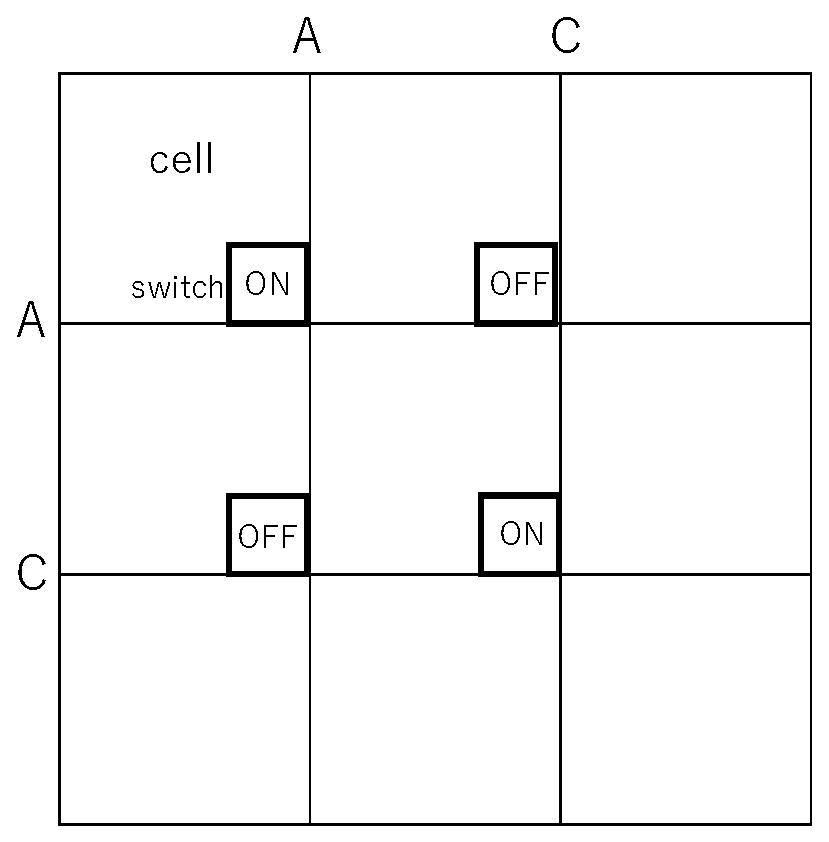
\includegraphics[keepaspectratio,scale=0.3]{fig/4/test_swich_a.eps}
\label{fig:test_swich_a}}
\subfigure[配列が一部一致の場合のスイッチ状態]{
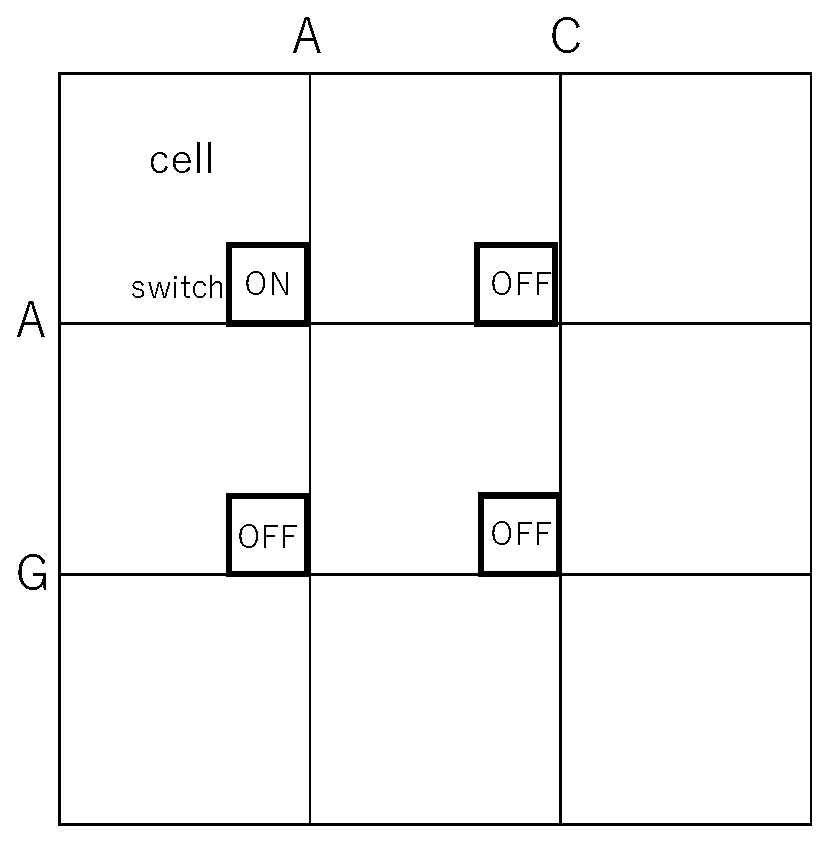
\includegraphics[keepaspectratio,scale=0.3]{fig/4/test_swich_b.eps}
\label{fig:test_swich_b}}
\subfigure[配列が完全不一致の場合のスイッチ状態]{
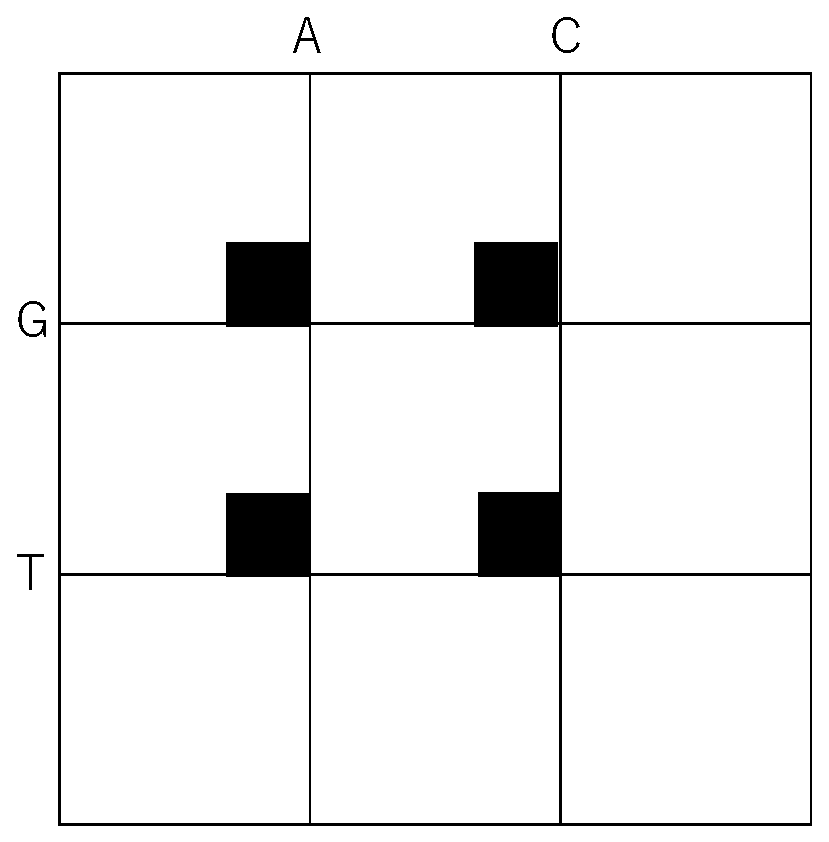
\includegraphics[keepaspectratio,scale=0.3]{fig/4/test_swich_c.eps}
\label{fig:test_swich_c}}
\caption{配列長N=2における光Race Logic arrayのスイッチ状態}
\label{fig:test_swich}
\end{center}
\end{figure}
\begin{figure}[t!]
\begin{center}
\subfigure[光Race Logic arrayへの光伝搬入力信号強度]{
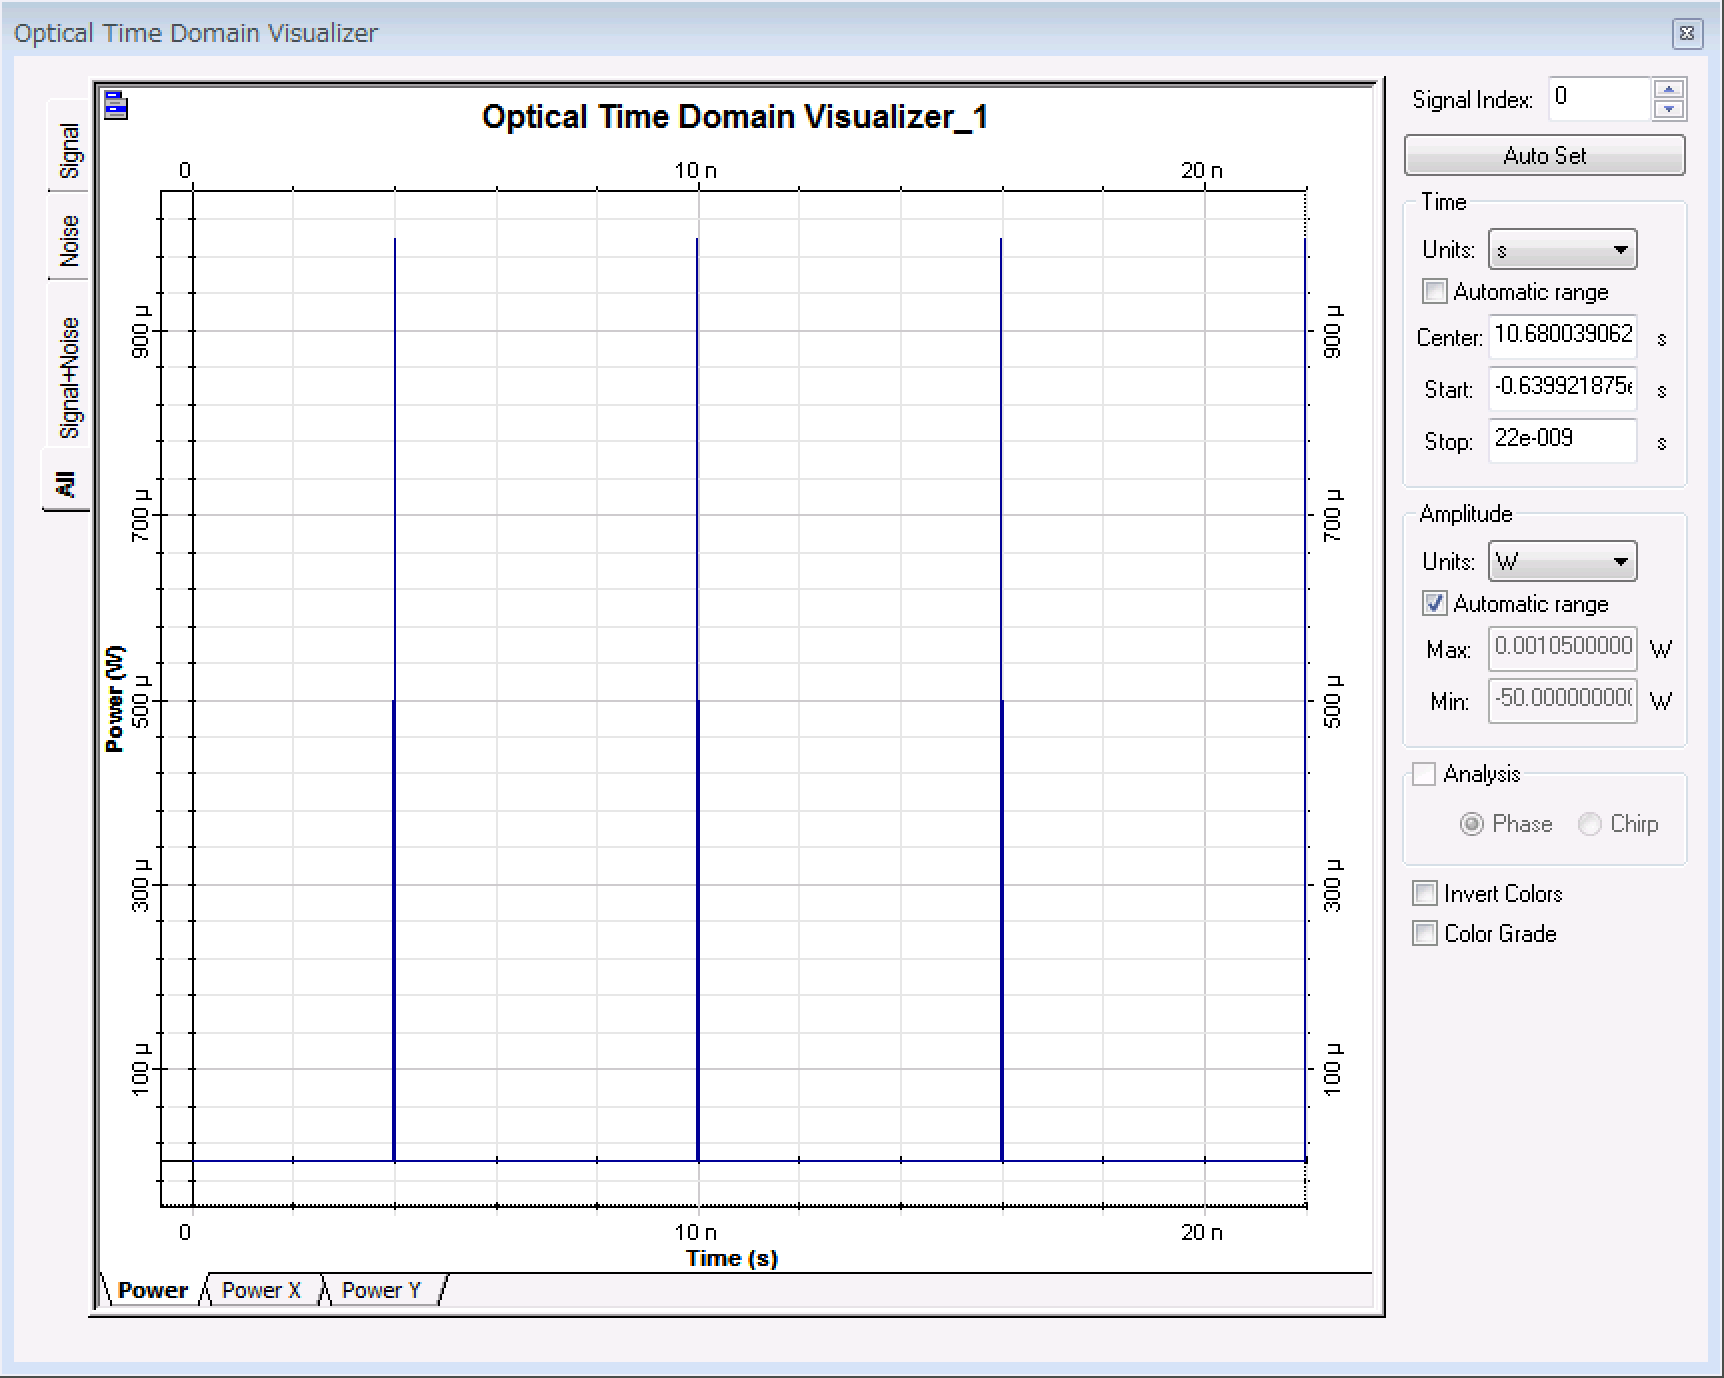
\includegraphics[keepaspectratio,scale=0.3]{fig/4/test_in.png}
\label{fig:test_in}}\\
\subfigure[光Race Logic arrayへの光伝搬出力信号強度]{
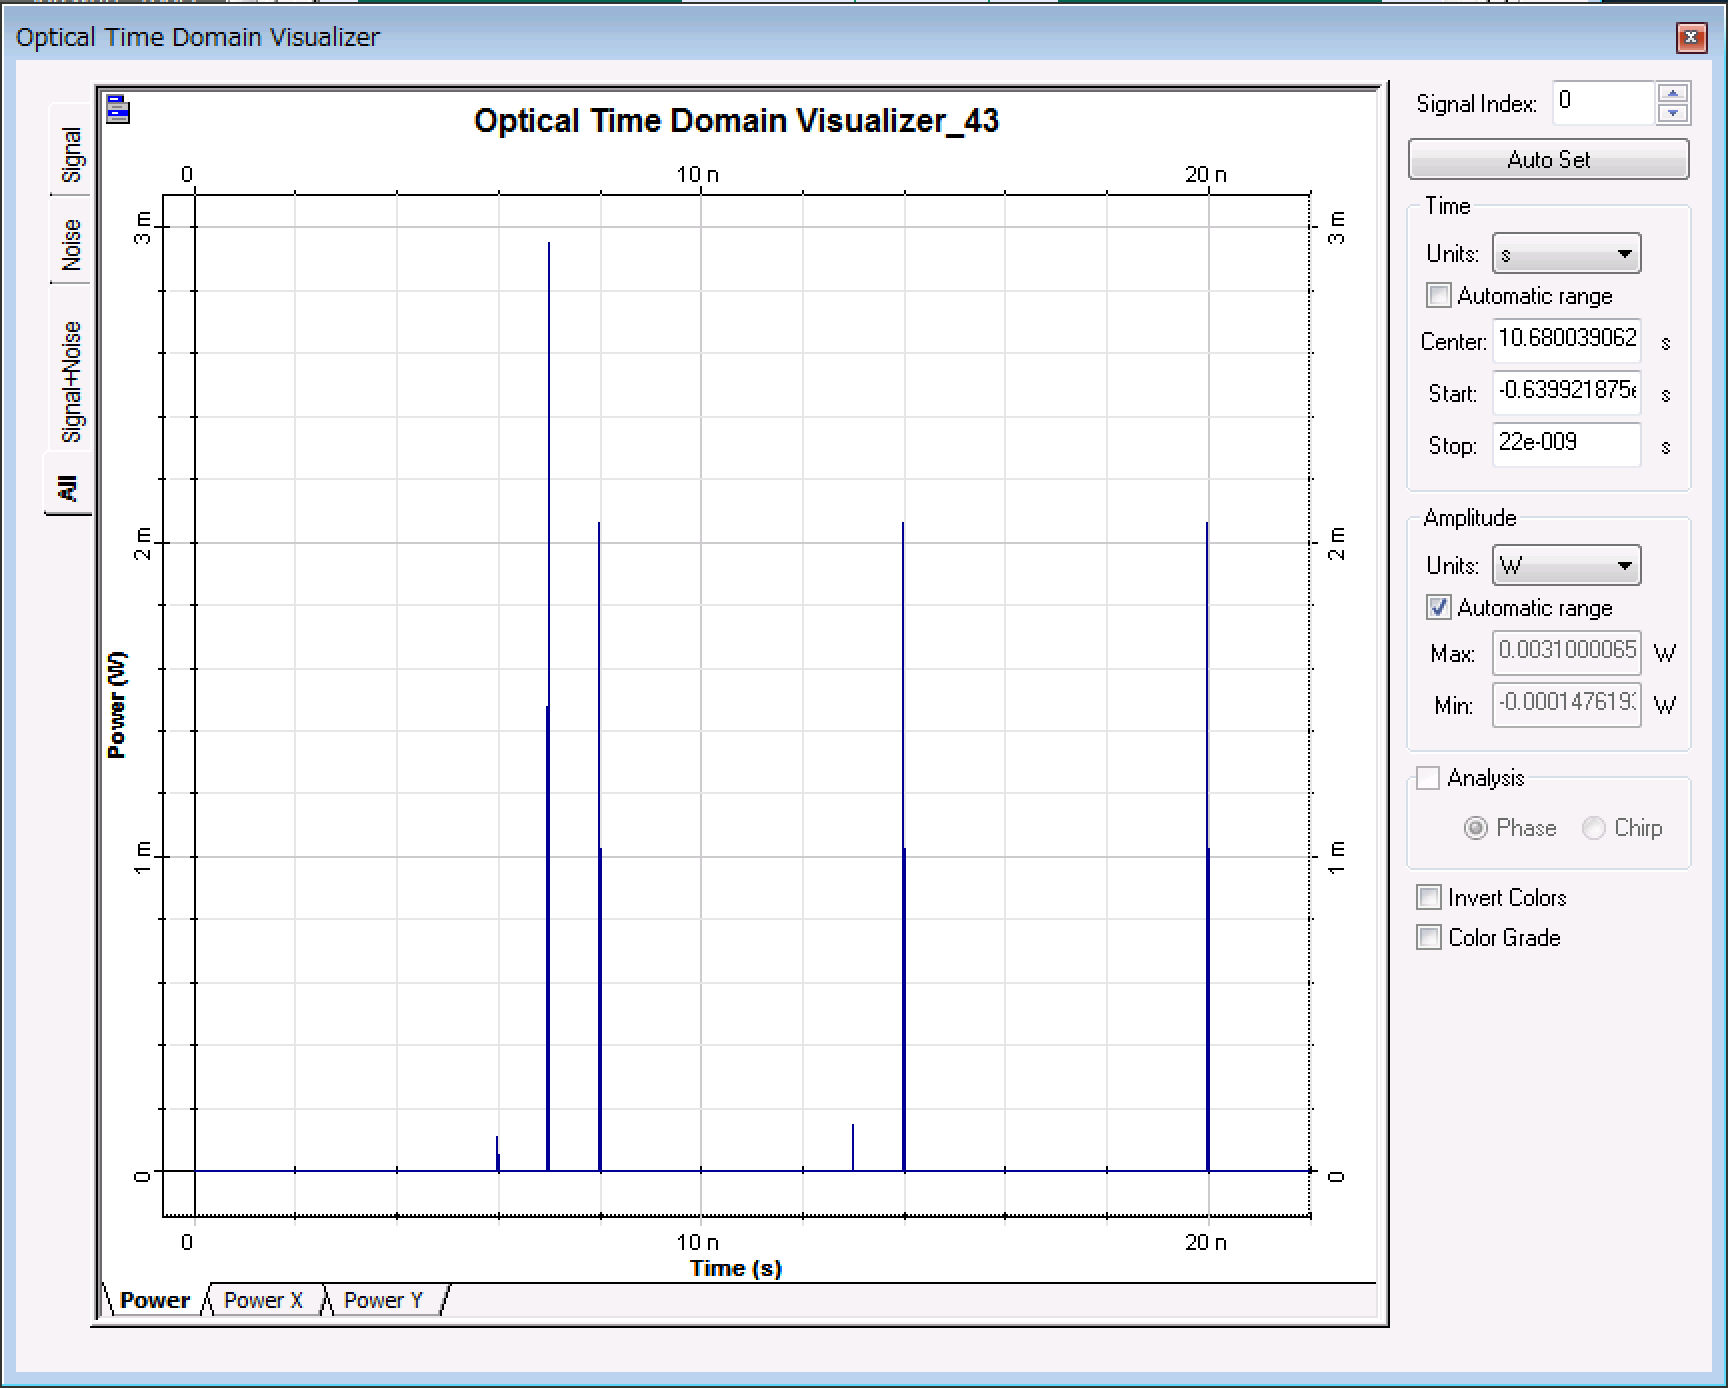
\includegraphics[keepaspectratio,scale=0.3]{fig/4/test_out.png}
\label{test_out}}
\caption{Optisystemによる機能検証結果}
\label{fig:test}
\end{center}
\end{figure}
今回のシミュレーションでは光遅延素子で発生する遅延時間が1nsと設定した.
また配列が一部一致の場合,取りうるスイッチ状態は図\ref{fig:test_swich_b}
だけではない.
今回のシミュレーションでは機能検証上の一例として図\ref{fig:test_swich_b}
の状態を取り扱う.

図\ref{fig:test_swich}のそれぞれの状態において,
出力から最初に観測される信号のタイミングは
入力から2ns後,3ns後,4ns後になると想定している.
図\ref{fig:test}の0ns〜8nsの区間は図\ref{fig:test_swich_a}の状態,
8ns〜14nsの区間は図\ref{fig:test_swich_b}の状態,
14ns〜20nsの区間は図\ref{fig:test_swich_c}の状態である.
図\ref{fig:test}を見ると,想定した動作をしているのが確認できた.

\section{評価}
本節では,提案した光Race Logic arrayの遅延時間,面積及び
一つのアラインメントを求める(以後,これを一計算と呼称する)毎のエネルギーが
配列長Nによってどう変化するかを見積るために
各項目を算出するモデルを構築し,評価を行う.
\subsection{遅延時間}
まず,光Race logic arrayに光伝搬信号が入射されてからarray内を伝搬し,
最初に出力された信号が受光器で検出されるまでの遅延時間を考える.
配列長Nの光Race logic arrayにおいて,最初に光伝搬信号が出力されるまでの回路遅延時間は
配列の組み合わせによって異なる.
二つの配列が完全に不一致の場合,最初に光伝搬信号が出力されるまでの回路遅延時間は
最長となる.
今回はこのワーストケースの遅延時間をモデル化した.

図\ref{fig:proposalcell}の構造より構築した遅延時間$T$のモデル式を式\ref{eq:latency}に示す.
\begin{eqnarray}
&&T = T_{wire}+2N \times T_{cell-pass}+T_{pd} \nonumber \\
&&T_{cell-pass} = T_{cell-wire}+T_{coupler}+T_{amp}+T_{splitter}+T_{switch-pass}
\label{eq:latency}
\end{eqnarray}

$T_{wire}はセル間の配線遅延時間,T_{cell-pass}は一つのセルを通過する遅延時間,T_{pd}は受光器の応答時間である.$
$T_{cell-pass}の内訳はT_{cell-wire}がセル内部の配線遅延,$
$T_{coupler}・T_{splitter}がそれぞれ光結合器・光分配器の遅延時間,$
$T_{amp}がアンプの遅延時間,T_{switch-pass}が光スイッチ遅延時間である.$
$T_{wire}とT_{cell-pass}が光伝搬入力信号が$光Race Logic array$を伝搬するために必要な時間,$
$T_{pd}が受光器が光出力信号を検出するまでに必要な時間である.$

\subsection{面積}
提案したセルの構成(図\ref{fig:proposalcell})より,
セル一つの面積$A_{cell}$を表すモデル式は式\ref{eq:cellArea}と書ける.
\begin{equation}
A_{cell} = A_{cell-wire}+A_{coupler}+A_{amp}+A_{splitter}+A_{switch}+2A_{delay}
\label{eq:cellArea}
\end{equation}

$A_{cell-wire}はセル内部の配線面積,A_{amp}がアンプの面積,$
$A_{coupler}・A_{splitter}はそれぞれ光結合器・光分配器の遅延時間,$
$A_{switch}が光スイッチの面積,A_{delay}は光遅延素子の面積である.$
このセルを基準セルとする.

基準セル並べてarrayを構成した時に,外周のセルはこの基準セルとは違う構成となる.
その差異の理解を助けるため,図\ref{fig:N=2}に配列長N=2の光Race Logic arrayの構造を示す.
この差異に留意しながら,配列長Nの光Race logic arrayの面積$A$をモデル化した.
モデル式を式\ref{eq:Area}に示す.
\begin{equation}
A = A_{wire}+N^2 \times A_{cell} + 2N \times (A_{delay}+A_{amp}) +A{ls}+A_{pd}
\label{eq:Area}
\end{equation}

$A_{wire}はセル間の配線面積,A{ls}は光源の面積,A_{pd}は受光器の面積である.$

\subsection{ー計算毎のエネルギー}
一計算毎のエネルギー$E$は式\ref{eq:Energy}によって求めることができる.
\begin{equation}
E=P*T+N^2 \times E_{v}
\label{eq:Energy}
\end{equation}

$P$は光Race Logic arrayの消費電力,
$T$は式\ref{eq:latency}で求めた一計算にかかる遅延時間,
$E_{v}は光スイッチの駆動に必要なエネルギーである.$

ここで本提案の光Race Logic arrayでの消費電力について考える.
この回路での消費電力は,式\ref{eq:power}に示すように
$光源の消費電力P_{ls}・アンプP_{amp}$の消費電力の二つのみで考えることができる.
\begin{equation}
P=P_{ls}+P_{amp}
\label{eq:power}
\end{equation}

$P$の値は,光Race Logic arrayが機能を担保できる値に設定しなければならない.
そこで,光Race Logic arrayの機能担保について具体的に見ていく.

配列長Nの光Race Logic arrayからの光伝搬出力信号強度$P_{out_NN}$は
式\ref{eq:power_out}と表せる.
\begin{equation}
P_{out\,N,N}=Loss_{NN}(P_{out\,(N-1),(N-1)}+P_{out\,(N-1),N}+P_{out\,N(N-1)})
\label{eq:power_out}
\end{equation}

$N \geq 0,P_{out\,-1,-1}=P_{ls},P_{out\,-1,0}=0,P_{out\,0,-1}=0である.$

$P_{out\,NN}$の値は配列の組み合わせ,即ちスイッチの状態によって大きく変化する.
光Race Logic arrayからの光伝搬出力信号は受光器で検出されなければならない.
よって,$P_{out\,NN}の最小値 \geq P_{r}となるようにP$の値を決定することが必要となる.

\subsubsection{ケーススタディ:配列長N=2における一計算毎のエネルギー}

